I problemi che verranno segnalati nel seguente capitolo non si sono presentati subito, ma solo quando si è testata l'accuratezza del modello per cui ci sono paragrafi in cui si parla di esso senza averlo ancora definito.
\section{Machine learning}
Usare un algoritmo scritto da un programmatore non è sempre la soluzione migliore in quanto bisogna definire tutti i parametri e i dati necessari alla risoluzione del problema. Infatti, esiste anche un'altra strategia cioè quella di far imparare ad una macchina come risolverlo. La prima cosa che viene spontaneo chiedersi è: come fa una macchina ad imparare? Gli psicologi ci insegnano che l’apprendimento consiste nell’acquisizione o modifica di conoscenze, comportamenti, abilità, valori ed esperienze che sono poi utilizzati per vivere la vita di tutti i giorni. Tramite l’apprendimento creiamo delle regole generali che sono assimilabili in modelli di apprendimento. Questi modelli ci indicano come comportarci in una determinata situazione, ad interagire con gli altri, come leggere, come socializzare e così via. L’apprendimento è un processo iterativo, che continua per tutta la vita e ci permette di migliorare le nostre conoscenze a seconda delle informazioni che raccogliamo. Lo stesso fanno le macchine: dai dati di \textit{input} che analizzano ricavano i modelli di apprendimento.\\
\newline
\section{Librerie utilizzate}
I \textit{package} usati per realizzare il progetto sono:
\begin{itemize}
	\item \textit{numpy, versione 1.17.4}, è una libreria che aggiunge supporto a grandi matrici e \textit{array} multidimensionali insieme a una vasta collezione di funzioni matematiche di alto livello per poter operare efficientemente su queste strutture dati;
	\item \textit{jams, versione 0.3.4}, è una libreria che legge file \textit{JSON} inerenti al mondo della musica;
	\item \textit{librosa, versione 0.8.0}, è una libreria per la musica e l'analisi audio. Fornisce gli elementi necessari per recuperare informazioni musicali;
	\item \textit{scipy, versione 1.4.1}, è una libreria di algoritmi e strumenti matematici che contiene moduli per l'ottimizzazione, per l'algebra lineare, elaborazione di segnali ed immagini e altro;
	\item \textit{matplotlib, versione 3.1.2}, è una libreria per la creazione di grafici;
	\item \textit{tensorflow, versione 2.1.0}, è una libreria utilizzata per il \textit{machine learning} che fornisce moduli sperimentati e ottimizzati, utili nella realizzazione di algoritmi per diversi tipi di compiti percettivi e di comprensione del linguaggio;
	\item \textit{keras, versione 2.3.1}, consente di implementazione algoritmi basati su reti neurali. Permette di sviluppare e prototipare in maniera semplice e veloce modelli nell’ambito del \textit{machine learning} e del \textit{deep learning}. Supporta come \textit{back-end} \textit{Tensorflow} ed è integrata in esso dalla versione 2.
\end{itemize}

\section{Set dati GuitarSet}
Fortunatamente, su Internet abbiamo trovato un \textit{dataset} di file audio di chitarra già pronto su cui lavorare. Il \textit{GuitarSet}, chiamato così dal suo creatore, è costituito dai file audio e dai suoi \textit{tab}.\\
\newline
Questo \textit{dataset} contiene trecentosessanta estratti di canzoni della durata di circa trenta secondi l'uno. Quest'ultime sono suonate da sei persone diverse che leggono gli stessi fogli musicali. I fogli musicali sono generati da una combinazione di:
\begin{itemize}
	\item \textbf{5 stili}: rock, cantautore, bossa nova, jazz e funk;
	\item \textbf{3 progressioni}: dodici bar blues, autumn leaves e pachelbel canon;
	\item \textbf{2 Tempi}: lento e veloce.
\end{itemize}
Gli estratti sono registrati sia con il \textit{pickup esafonico} che con un microfono a condensatore \textit{Neumann U-87}.
Ci sono tre registrazioni audio per ogni estratto:
\begin{itemize}
	\item \textbf{hex}: file .\textit{wav} originali a sei canali dal \textit{pickup esafonico};
	\item \textbf{hex\_cln}: file .\textit{wav} con rimozione delle interferenze applicata;
	\item \textbf{mic}: registrazione monofonica dal microfono di riferimento.
\end{itemize}
Noi abbiamo usato registrazioni di tipo \textbf{mic} perchè sono quelle che più si avvicinano al caso delle registrazioni tramite microfono dello \textit{smartphone}.\\
\newline
Ciascuno dei trecentosessanta estratti ha anche un file .\textit{jams} che memorizza sedici annotazioni:
\begin{itemize}
	\item Intonazione:
	\begin{itemize}
		\item 6 annotazioni \textit{pitch\_contour} (1 per stringa)
		\item 6 annotazioni \textit{midi\_note} (1 per stringa)
	\end{itemize}
	\item Beat e tempo:
	\begin{itemize}
		\item 1 annotazione \textit{beat\_position}
		\item 1 annotazione del tempo
	\end{itemize}
	\item Accordi:
	\begin{itemize}
		\item 2 annotazioni di accordi (istruite ed eseguite)
	\end{itemize}
\end{itemize}
Noi useremo le annotazioni \textit{midi\_note}, da cui prenderemo le \textit{tab}.
\subsection{Ricavare le tab dai file .jams}
Innanzitutto calcoliamo il numero di \textit{frame} per ogni \textit{file} audio, così da poter ricavare un'immagine completa e le corrispondenti \textit{tab} per ogni \textit{frame}. Per calcolare l'istante di tempo per ogni \textit{frame} utilizziamo la funzione \textit{get\_times()}:
\vspace*{2ex}
\pythonexternal{./codes/times.py}
\vspace*{2ex}
\noindent Adesso che, per ogni \textit{file} audio, abbiamo una divisione in \textit{frame} di cui conosciamo gli istanti di tempo esatti, possiamo estarre dai file .\textit{jams} del \textit{dataset} le \textit{tab} corrispondenti.\\ Più precisamente, dai file .\textit{jams} prendiamo le note \textit{MIDI} e creiamo una matrice 6x19 dove il sei rappresenta il numero di corde mentre il diciannove rappresenta il numero di tasti.
\vspace*{2ex}
\begin{figure}[H]
	\centering
	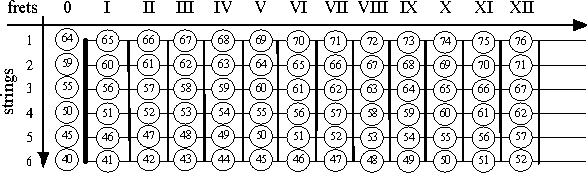
\includegraphics[scale=0.65]{./images/img11.png}
\end{figure}
\noindent Ogni tasto della matrice ha un valore \textit{MIDI} che varia da 40 a 82.
\vspace*{2ex}
\pythonexternal{./codes/matrixMidi.py}
\vspace*{2ex}
\noindent Ad ogni matrice sostituiamo i valori \textit{MIDI} con una matrice della stessa dimensione in cui ci sono solo uni o zeri a seconda dei valori \textit{MIDI} che il \textit{file} .\textit{jams} ci ha restituito. Ad esempio, dato un \textit{frame}, se dal file .\textit{jams} leggiamo che sono state suonate le note 40 della sesta corda, 60 della seconda corda e 67 della prima, avremo la seguente matrice:
\vspace*{2ex}
\pythonexternal{./codes/matrixUniZeri.py}
\noindent Queste matrici, da ora in avanti, saranno chiamate \textit{labels} e verranno usate come \textit{target y} del modello, per questo è molto importante avere una mappatura di numeri interi "categorica", per cui useremo la codifica \textit{one-hot}, cioè si può trovare un solo "1" in ogni riga. Per finire, aggiungiamo altre due colonne in testa alle labels che serviranno a capire se la corda è stata suonata o meno (colonna 0) e se si, se è stata suonata a vuoto oppure o no (colonna 1).\\
\newline
Di conseguenza, la matrice finale di dimensione 6x21 è la seguente:
\vspace*{2ex}
\pythonexternal{./codes/matrixUniZeriFinale.py}
\vspace*{2ex}
\noindent Il codice che esegue quanto abbiamo appena descritto è il seguente:
\vspace*{2ex}
\pythonexternal{./codes/labels.py}
\subsection{Ricavare le immagini dai file audio}
Dopo esserci ricavati le \textit{labels} per ogni \textit{frame}, dobbiamo trovare un modo per far "imparare" al modello che un frammento di audio sia associato al corrispondente \textit{label}.
Grazie alla libreria \textit{librosa} possiamo analizzare e manipolare il suono, vedere lo spettrogramma della trasformata a Q costante e ricavare per ogni \textit{file} audio un'immagine.\\
Per esempio, questo è lo spettrogramma della trasformata a Q costante di un audio del \textit{dataset}.
\begin{figure}[H]
	\centering
	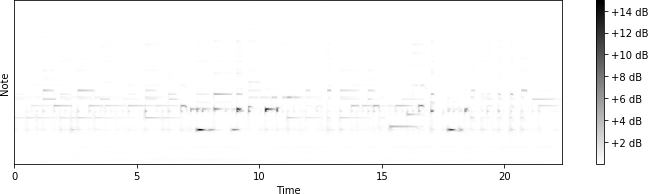
\includegraphics[scale=0.60]{./images/img7.png}
\end{figure}
\noindent Per utilizzare al meglio il modulo \textit{librosa.cqt()}, dobbiamo impostare alcuni parametri:
\begin{itemize}
	\item \textbf{sr\_downs}: il numero di campioni al secondo del segnale di ingresso;
	\item \textbf{hop\_length}: il numero di campioni tra i fotogrammi;
	\item \textbf{n\_bins}: il numero di bande di frequenza nello spettrogramma risultante;
	\item \textbf{bins\_per\_octave}: il numero di bande di frequenza per ogni ottava.
\end{itemize}
\textbf{Problemi riscontrati:} le funzioni per caricare il \textit{file} audio e la \textit{cqt} restitiscono dei valori negativi e non scalati, per questo bisogna effettuare delle operazioni sulle matrici che potrebbero alterare il risultato. Inoltre, la scelta dei parametri di \textit{simple rate} e \textit{n\_bins} influenzano l'accuratezza del modello. \\
\newline
\textbf{Soluzioni provate:}
\begin{itemize}
	\item Abbiamo avuto la necessità di scrivere delle funzioni per convertire i valori della matrice calcolata. Dunque, è stata ridimensionata in modo che si trovi nell'intervallo 0-255 e poi normalizzata nell'intervallo 0-1;
	\item All'inizio l'audio è stato campionato a 44100Hz perchè è la stessa frequenza usata nel \textit{dataset}. Le immagini generate avevano una frequenza delle note maggiore di quella che avrebbero dovuto avere. Infatti, nella figura in alto la parte scura era meno spessa. Questo provocava delle imprecisioni perchè la rete non riusciva a riconoscere la nota corretta;
	\item Il valore iniziale scelto di \textit{n\_bins} è stato 96. Questo influenzava le dimensioni dell'immagine in quanto è il valore della sua lunghezza e risultava troppo piccola.
\end{itemize}
\textbf{Soluzione finale:} le scelte finali sono ricadute rispettivamente su 22050Hz come \textit{simple rate} e su 192 come \textit{n\_bins} perchè dopo aver effettuato diverse ricerche, in ambito di manipolazione del suono, è consigliato utilizzare questi valori. Per quanto riguarda il ridimensionamento abbiamo usato le funzioni \textit{librosa.util.normalize()} e \textit{np.abs()} subito dopo aver caricato i file audio invece di manipolare le matrici in seguito.
\vspace*{2ex}
\pythonexternal{./codes/librosa.py}
\vspace*{2ex}
\noindent In particolare, una volta che l'audio è un oggetto dati \textit{librosa}, \textit{Python} lo vede come un numpy \textit{array} e quindi possiamo evitare di salvarci fisicamente dei classici \textit{file} immagini \textit{.jpeg} o \textit{.png} e continuare a lavorare con le matrici.\\
\newline
I dati (\textit{images} e \textit{labels}) di ogni \textit{file} audio sono stati compressi in archivi .\textit{npz} per organizzare meglio il \textit{dataset} da dare come \textit{input} al modello.
\vspace*{2ex}
\pythonexternal{./codes/store.py}
\vspace*{2ex}
\subsection{Pre-elaborare i dati}
Carichiamo i \textit{file} .\textit{npz} salvati in precedenza.\\
\newline
\textbf{Problemi riscontrati:} mentre lavoravamo con il modello ci siamo resi conto che usare una finestra di 1s risultava essere troppo ampia. Se nell'immagine ci sono troppe note e la rete deve riconoscerne poche, non riesce a farlo. Infatti, se non viene scelta  correttamente la finestra, l'accuratezza del modello è molto bassa e dopo appena 15 epoche la rete non tende più ad imparare.
\begin{figure}[H]
	\centering
	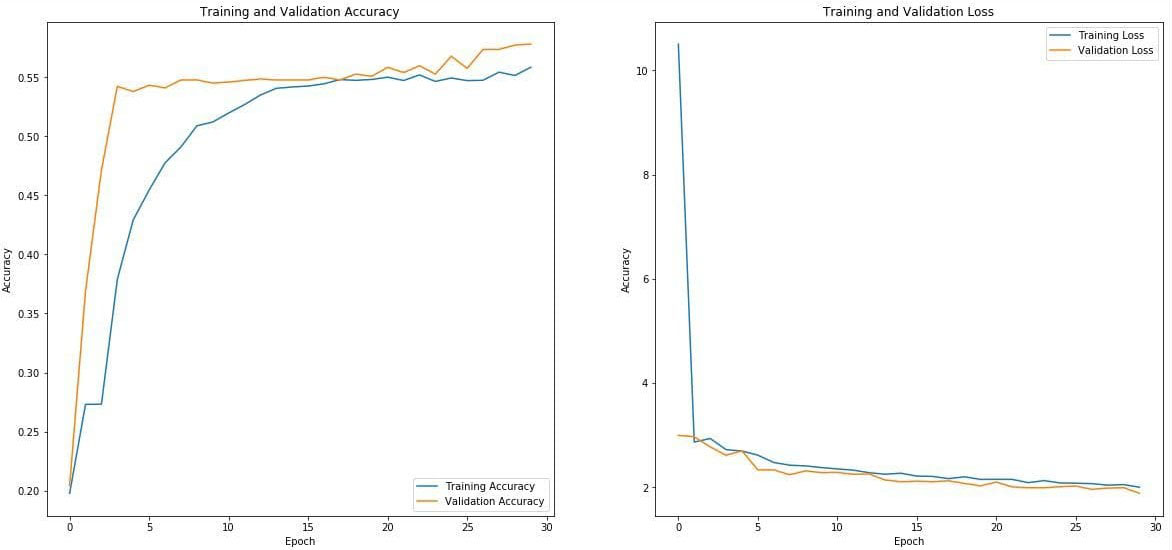
\includegraphics[scale=0.5]{./images/img28.jpg}
\end{figure}
\textbf{Soluzioni provate:}
\begin{itemize}
	\item Abbiamo provato finestre di grandezza compresa tra 0.1s e 0.3s.
\end{itemize}
\textbf{Soluzione finale:} si è visto, sperimentalmente, che un buon arco di tempo per riconoscere una nota è 200ms che, nel nostro caso, corrispondono ad una finestra di nove righe della matrice dell'immagine.\\
\newline
Di conseguenza, quello che dobbiamo fare non è altro che associare, per ogni \textit{frame}, una \textit{label} e un'\textit{immagine} di nove righe (192x9), senza dimenticare di aggiungere un \textit{padding} (quattro zeri nell'\textit{array}, sia all'inizio che alla fine, con la funzione \textit{np.pad()}) perchè così l'ultimo valore, della finestra di nove righe, risulta essere congruo con gli altri.\\
\newline
\begin{figure}[H]
	\centering
	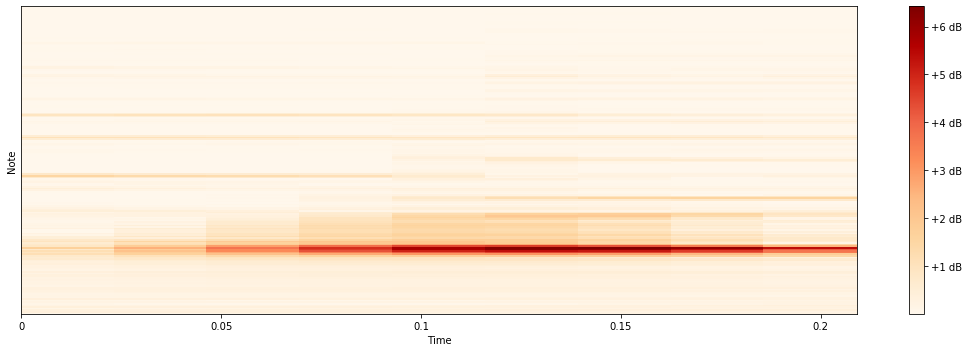
\includegraphics[scale=0.40]{./images/img8.png}
\end{figure}
\noindent Il codice che esegue quanto abbiamo appena descritto è il seguente:
\vspace*{2ex}
\pythonexternal{./codes/preElaborazionedati1.py}
\vspace*{2ex}
Una volta ottenuto l'\textit{array}, chiamato (\textit{training\_data}), di tutte le \textit{images} e i \textit{labels} dei \textit{file} audio, e assegnati rispettivamente le variabili \textit{X} e \textit{y}, lo mescoliamo in modo da avere più imprevedibilità. Infine, suddividiamo questi dati nel seguente modo:
\begin{itemize}
	\item 10\% dei dati li usiamo per la \textit{validation}
	\item 10\% dei dati li usiamo per i \textit{test}
	\item 80\% dei dati li usiamo per il \textit{traning}
\end{itemize}
Il \textit{traning set} lo utilizziamo per costruire il modello, il \textit{validation set} per validare i parametri dei \textit{layer} della rete neurale mentre il \textit{test set} per determinare l'accuratezza.\\
\newline
Il codice è il seguente:
\vspace*{2ex}
\pythonexternal{./codes/preElaborazionedati2.py}
\vspace*{2ex}
\section{Modello della rete}
La difficoltà nell’apprendere i meccanismi di implementazione su \textit{Keras} sono ridotti al minimo grazie alla vasta documentazione presente, arricchita da numerosi esempi sulle più utilizzate configurazioni inerenti il \textit{machine learning}, come le \textit{CNN} (Convolutional Neural Network).
Le operazioni di calcolo matriciali possono essere accelerate sia tramite \textit{CPU}, che \textit{GPU} (su \textit{hardware} \textit{Nvidia} con supporto \textit{CUDA}). Nel nostro caso è stata utilizzata una \textit{GPU} in modo da sfruttare direttamente la sua potenza parallela contenute nelle schede video recenti.
\vspace*{2ex}
\pythonexternal{./codes/gpu.py}
\vspace*{2ex}
\noindent Le caratteristiche e i vantaggi che ci hanno portato ad utilizzare \textit{Keras} nell’ambito del progetto sono:
\begin{itemize}
	\item \textbf{semplicità}: a differenza di altre \textit{API}, è possibile realizzare modelli complessi scrivendo meno righe di codice, mantenendo nel contempo chiarezza nello sviluppo. Tutto ciò consente allo sviluppatore di mantenere nel tempo il codice in maniera agevole;
	\item \textbf{modularità}: un modello in \textit{Keras} è inteso come una sequenza o un grafo di singoli, compatti e completamente configurabili moduli, che possono lavorare in sinergia tra loro con il minimo numero di restrizioni possibili. Ciò rende il codice estremamente flessibile;
	\item \textbf{estensibilità}: in base alle esigenze dello sviluppatore, è possibile aggiungere facilmente nuovi moduli (ad esempio classi e funzioni) ad un progetto preesistente.
\end{itemize}
\subsection{Uso di Keras}
Prima di dare in \textit{input} al modello il \textit{traning set} e il \textit{validation set}, dobbiamo fare delle modifiche alla dimensione del numpy \textit{array} delle immagini \textit{X} in quanto il modello si aspetta una dimensione di \textit{input} di \textit{BATCH} x 192 x 9 x 1.
\begin{itemize}
	\item \textit{BATCH} sono la quantità di valori dell'intero \textit{training set};
	\item 192 è l'altezza dell'immagine (H);
	\item 9 è la lunghezza dell'immagine (W);
	\item 1 ci indica che l'immagine è in bianco e nero.
\end{itemize}
La \textit{y} non ha bisogno di modifiche perchè le dimensioni sono già quelle corrette cioè ha dimensione \textit{BATCH} x 21 x 6.\\
\newline
Il codice che esegue quanto abbiamo appena descritto è il seguente:
\vspace*{2ex}
\pythonexternal{./codes/modelloFinale1.py}
\vspace*{2ex}
A questo punto definiamo il modello con l'aggiunta dei seguenti \textit{layers}:
\begin{itemize}
	\item \textbf{Conv2D}: mette in evidenza le caratteristiche interessanti dell'immagine. Parametri di \textit{input}: numero di filtri, grandezza filtri, \textit{input shape} e funzione di attivazione;
	\item \textbf{MaxPooling2D}: riduce la dimensione dell'immagine, elimina le informazioni inutili mantenendo quelle più importanti;
	\item \textbf{Dropout}: elimina una percentuale di dati casuali. Ad esempio, elimina rumori di sottofondo e mantiene le informazioni più importanti;
	\item \textbf{Flattern}: appiattisce il tensore e rimuove tutte le dimensioni;
	\item \textbf{Dense}: crea un \textit{layer} di neuroni, ognuno dei quali connesso ad ogni uscita del \textit{layer} precedente;
	\item \textbf{Reshape}: determina la dimensione di uscita. In questo caso è 6x21;
	\item \textbf{Activation}: la funzione di attivazione è una "porta" matematica tra l'\textit{input} che alimenta il neurone corrente e il suo \textit{output} che va allo strato successivo.
\end{itemize}
L'unità lineare rettificata (\textit{ReLU}) è la funzione di attivazione più comunemente utilizzata nel \textit{deep learning}. La funzione restituisce 0 se l'\textit{input} è negativo, ma per qualsiasi \textit{input} positivo, restituisce quel valore.\\
La funzione \textit{softmax} è molto utilizzata in statistica e consente di gestire un vettore di uscita normalizzato di n elementi, dove ogni elemento può valere da 0 ad 1 e la somma di tutti gli elementi è pari ad 1. In sostanza il nostro vettore di uscita sarà in una forma simile a quella \textit{one-hot} e ogni posizione corrisponderà alla probabilità (normalizzata) che l’immagine appartenga a quella specifica classe. La somma di tutte le probabilità sarà 1 = 100\%.
\begin{figure}[H]
	\centering
	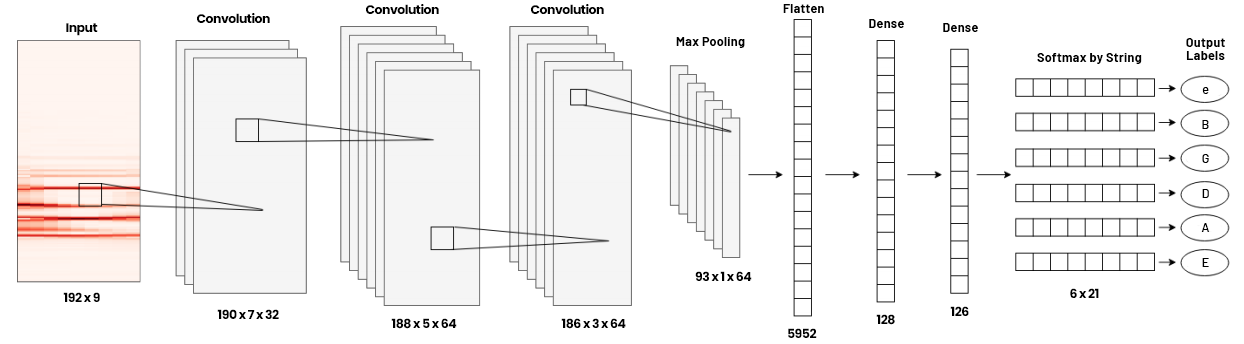
\includegraphics[scale=1.4]{./images/model.png}
\end{figure}
\noindent Per compilare il modello abbiamo scelto come ottimizzatore l'algoritmo \textit{Adadelta} che utilizza un metodo di discesa del gradiente stocastico basato sul tasso di apprendimento adattivo per dimensione per affrontare l'inconveniente del continuo declino dei tassi di apprendimento durante la formazione e la necessità di un tasso di apprendimento globale selezionato manualmente.\\
Il codice è il seguente:\\
\newline
\vspace*{2ex}
\pythonexternal{./codes/modelloFinale3.py}
\vspace*{2ex}
\noindent La funzione \textit{summary()} ci descrive il modello:
\vspace*{2ex}
\pythonexternal{./codes/modelloFinale5.py}
\vspace*{2ex}
\noindent In particolare, per il modello abbiamo usato delle funzioni personalizzate per la funzione di attivazione finale del modello (\textit{sofmax\_by\_string}), per la funzione obiettivo \textit{loss} (\textit{catcross\_by\_string}) e per le metriche di accuratezza (\textit{avg\_acc}) che devono essere valutate dal modello durante l'addestramento.\\
Esse permettono di utilizzare la funzione di attivazione \textit{softmax} e la funzione di perdita \textit{categorical\_crossentropy} per ogni stringa, e alla fine concatenare i sei risultati in un unico valore.\\
\newline
Il codice che esegue quanto abbiamo appena descritto è il seguente:
\vspace*{2ex}
\pythonexternal{./codes/modelloFinale2.py}
\vspace*{2ex}
\noindent Per avviare l'addestramento del modello eseguiamo la funzione \textit{model.fit()} dove indichiamo con \textit{batch\_size} il numero di campioni per ogni aggiornamento del gradiente e con \textit{epochs} il numero di iterazioni sul quale il modello deve effettuare il \textit{training}. In questo modo partirà la fase di addestramento che andrà ad affinare sempre di più le performance del modello.\\
\newline
Il codice che esegue quanto abbiamo appena descritto è il seguente:
\vspace*{2ex}
\pythonexternal{./codes/modelloFinale4.py}
\subsection{Addestramento del modello}
Dopo diverse prove sperimentali, abbiamo deciso di eseguire il modello per cinquecento epoche:
\begin{figure}[H]
	\centering
	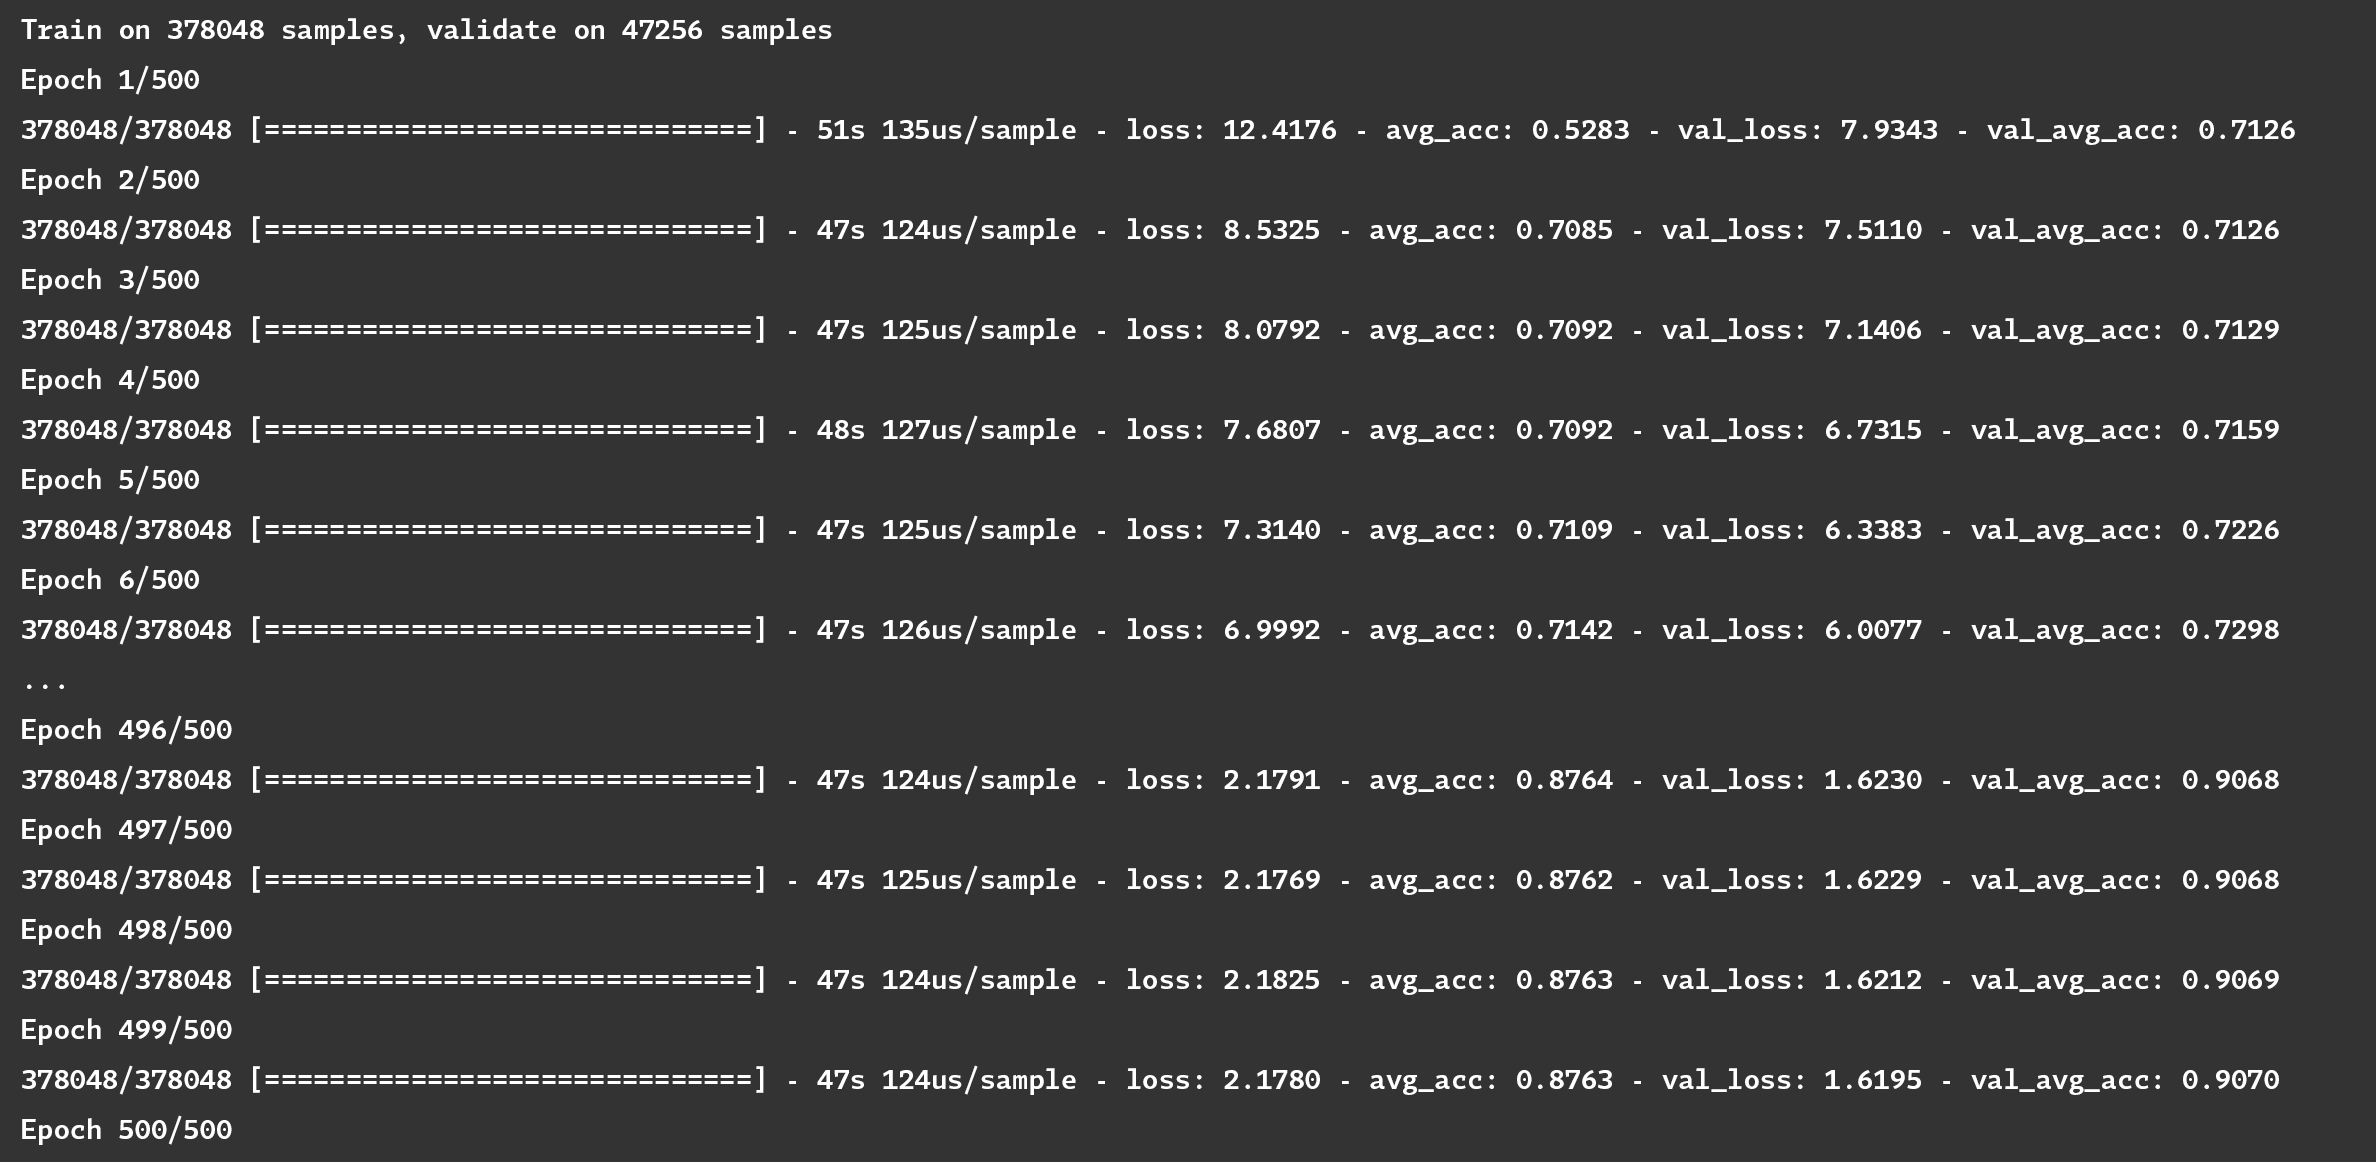
\includegraphics[scale=0.8]{./images/storia.png}
\end{figure}
\noindent Come si può notare dal \textit{log}, un’epoca (cioè l’addestramento eseguito su un intero \textit{dataset} di 378048 immagini) viene eseguita in circa 47 secondi, usando mediamente 124 microsecondi per immagine. Questo è il risultato ottenuto utilizzando una \textit{GPU NVIDIA RTX 2060}.\\
\newline
Questo modello raggiunge una precisione di circa 0,87 su 1 (o 87\%) e una perdita del 2\% sui dati di addestramento. Invece, sui dati di validazione la precisione supera lo 0,90 (90\%) e raggiunge una perdita del 1,6\% sui dati di validazione. I \textit{loss} sono la media delle perdite sui dati di \textit{batch} di addestramento.\\
\newline
Il grafico sottostante ci fa comprendere meglio i risultati:
\begin{figure}[H]
	\centering
	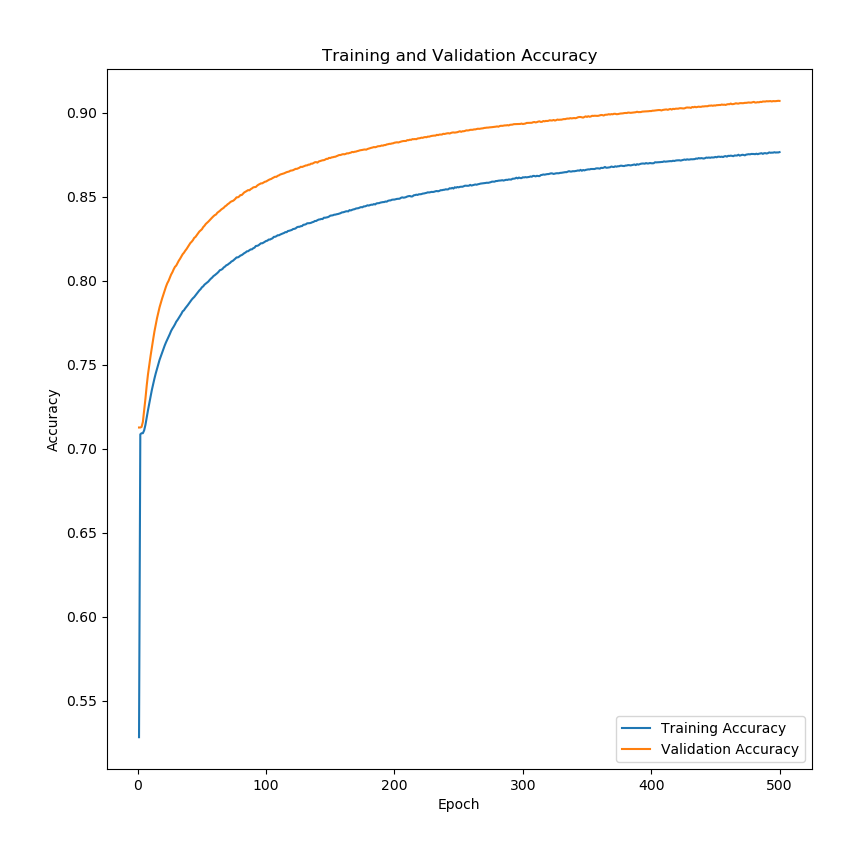
\includegraphics[scale=0.40]{./images/plot.png}
\end{figure}
\begin{figure}[H]
	\centering
	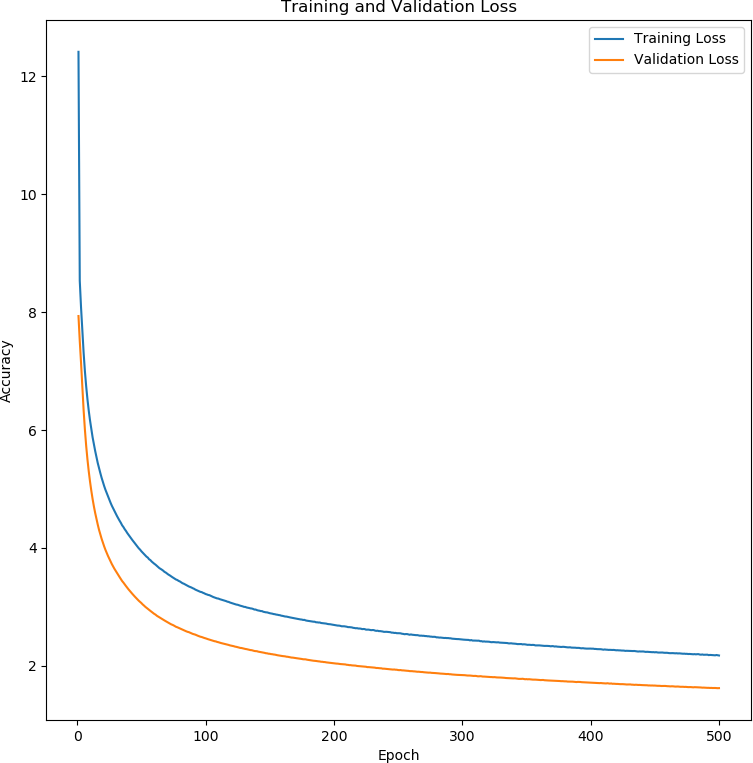
\includegraphics[scale=0.40]{./images/plot2.png}
\end{figure}

\section{Valutazione del modello}
Abbiamo eseguito diversi \textit{test} per mettere alla prova il modello utilizzando il \textit{training test}. La matrice \textit{Answer} è la \textit{y} corrispondente alla \textit{X} data come \textit{input} alla \textit{predict}. Invece, la \textit{Prediction} corrisponde all'\textit{output} della rete. Il valore più grande della riga corrisponde a dove secondo il modello ci debba essere "1".\\
\newline
Di seguito riportiamo un esempio:
\vspace*{2ex}
\pythonexternal{./codes/test.py}
\vspace*{2ex}
\noindent Abbiamo confrontato le prestazioni del modello sul \textit{dataset} di prova e i risultati sono stati quelli previsti. Infatti, l'accuratezza e la perdita dei dati di \textit{test} sono molto simili a quelli dei dati di validazione. Quello che otteniamo è un errore del 10\% (quindi un'\textit{accuracy} del 90\%).
\vspace*{2ex}
\pythonexternal{./codes/valutazione.py}
\vspace*{2ex}

Il codice che esegue quanto abbiamo appena descritto è il seguente:
\vspace*{2ex}
\pythonexternal{./codes/accuratezza.py}
\vspace*{2ex}